\chapter{مفاهیم پایه}

در این فصل به معرفی تکنولوژی و فریمورک های به کار رفته در پروژه میپردازیم.

\section{Firecracker}
در قلب پروژه Firecracker قرار دارد. Firecracker یک مانیتور ماشین مجازی است که از KVM استفاده می‌کند و
وظیفه اش ساخت و مدیریت ماشین های مجازی است.
Firecracker توسط تیم وب سرویس آمازون توسعه داده شده و در پروژه Fargate و Lambda این شرکت نیز استفاده شده است.

\begin{figure}[h]
    \centering
    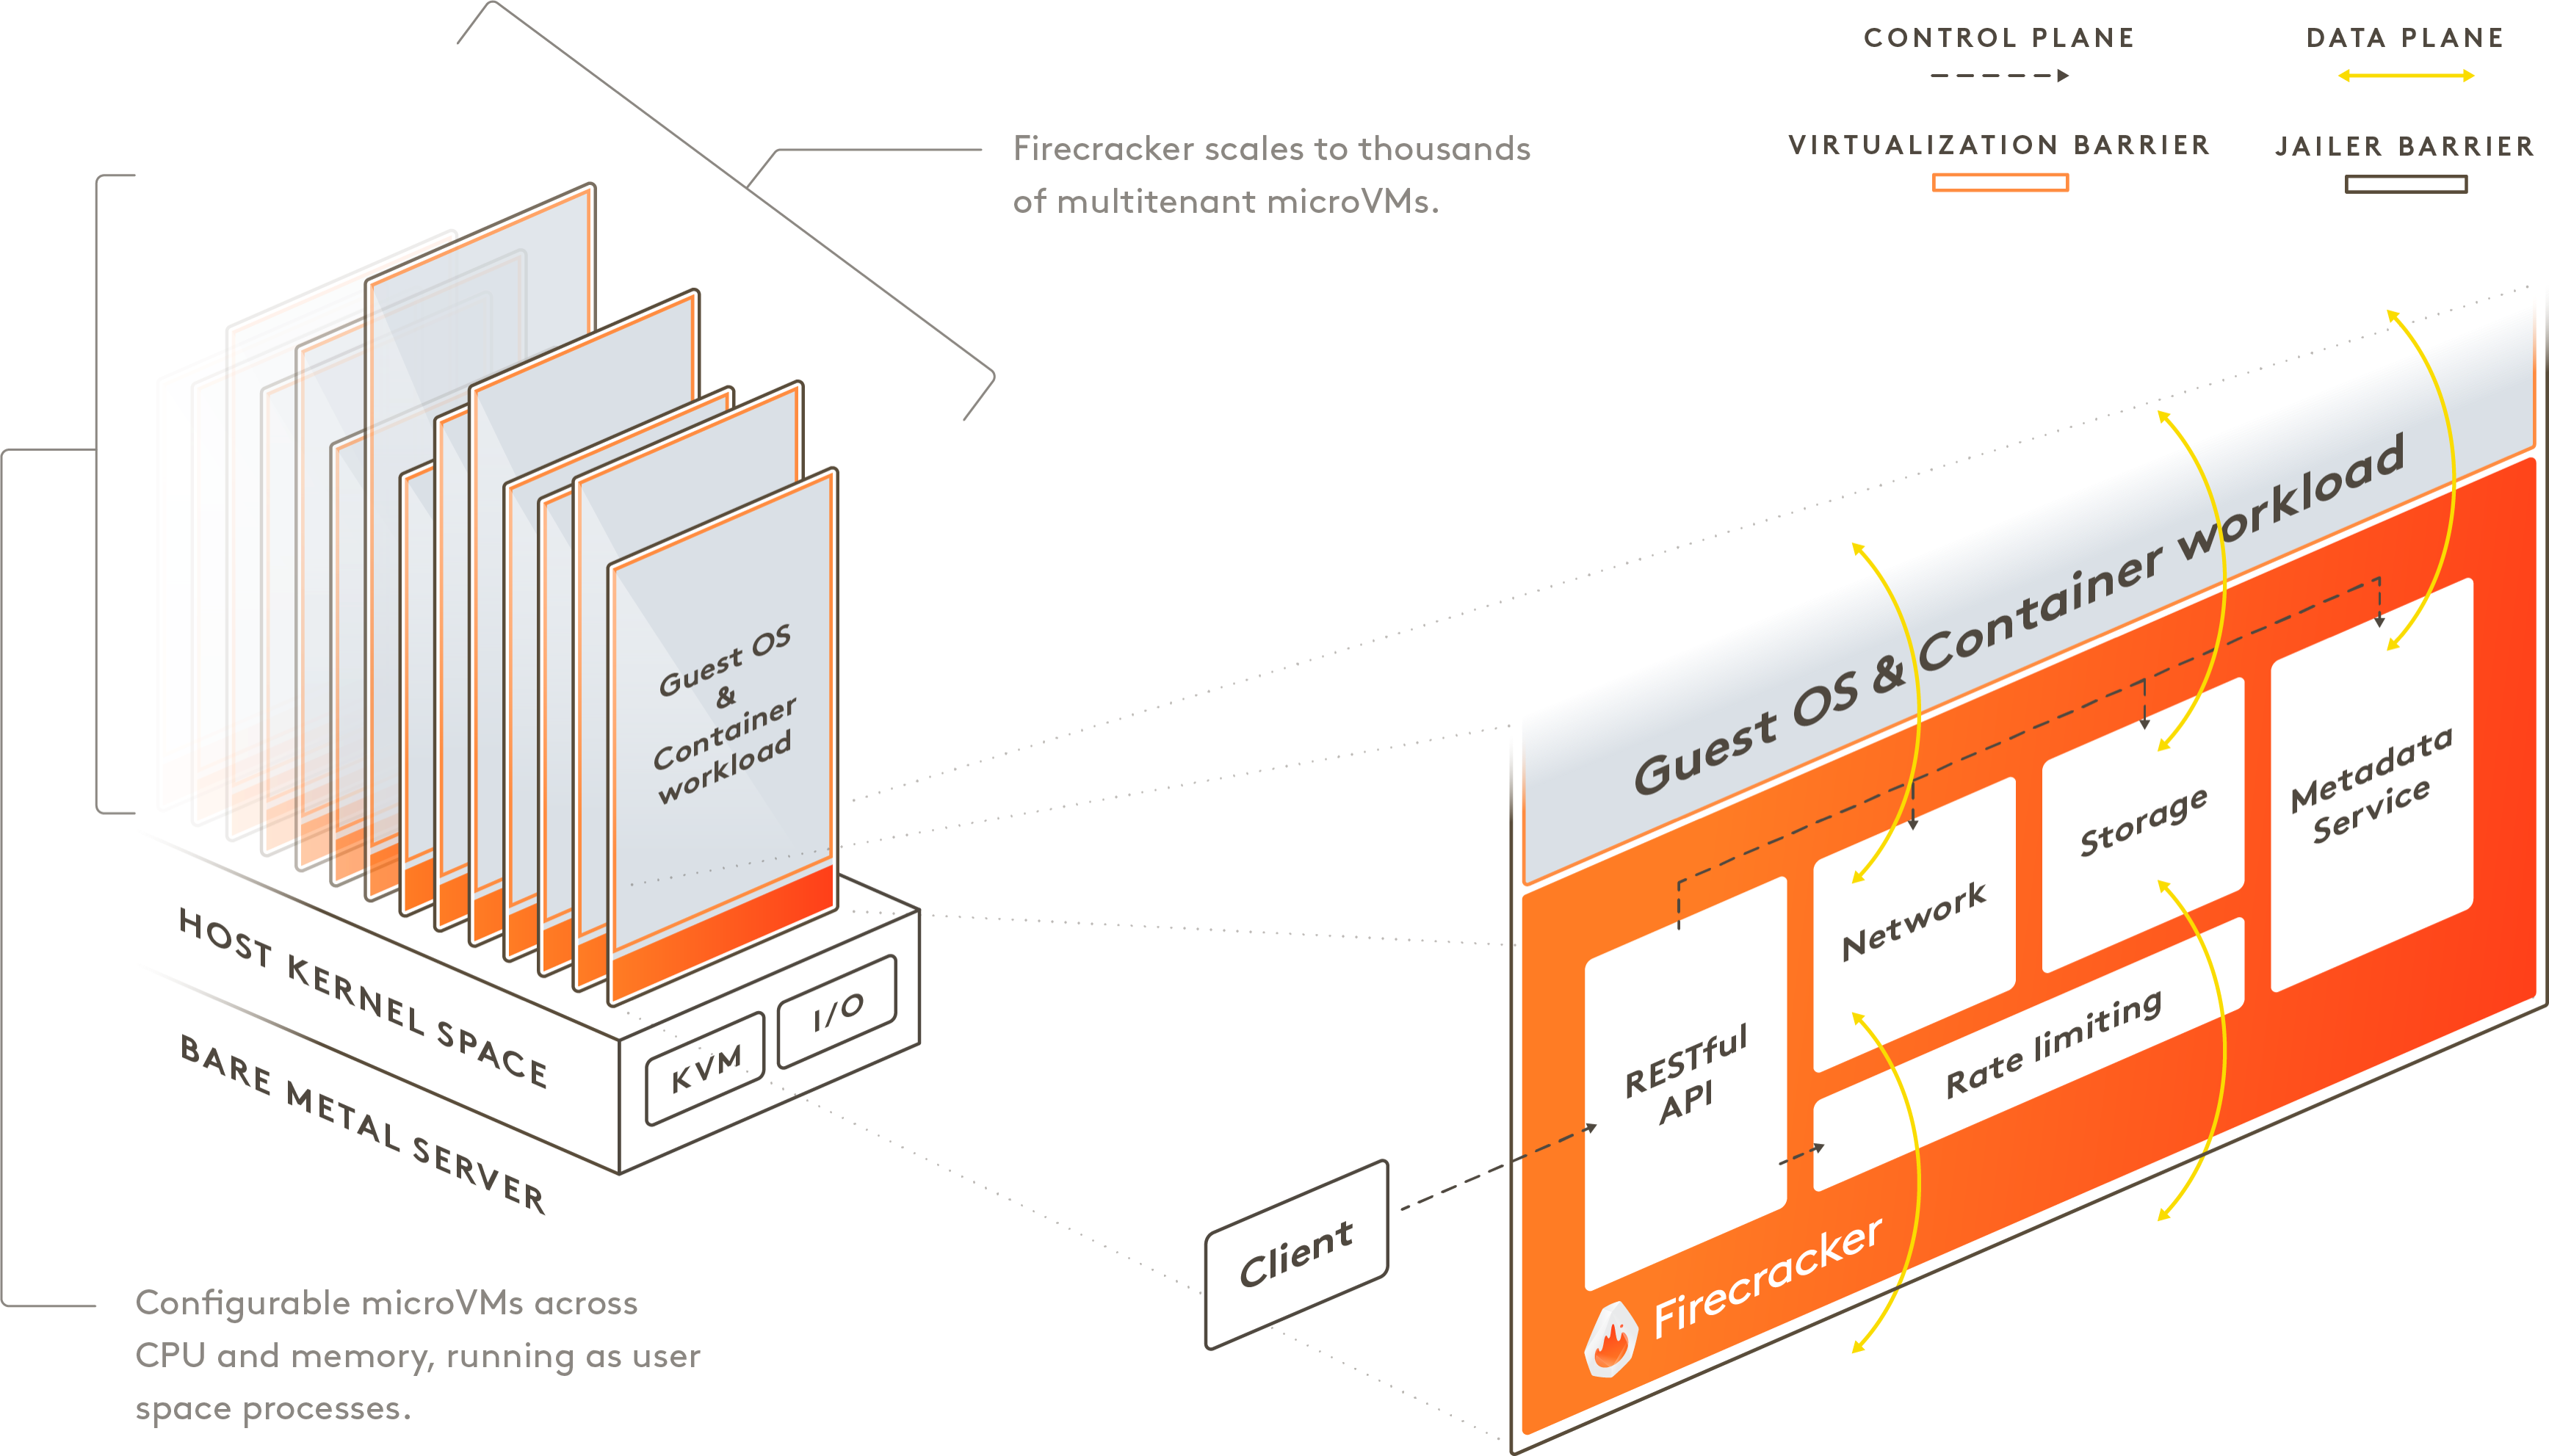
\includegraphics[width=0.7\textwidth]{./2-Basic-Concepts/firecracker-diagram.png}
    \caption{نمایی از ساختار Firecracker}
    \label{fig:firecracker}
\end{figure}

\section{Go Fiber}
زبان استفاده شده در میکروسرویس ها Go می‌باشد که توسط گوگل توسعه داده شده و از فریمورک Fiber استفاده شده که برای ساده تر شدن routing و middleware استفاده شده است.
از دلایل استفاده از Go میتوان به سادگی و سرعت بالا اشاره کرد. همچنین این زبان در مسائل concurrency ابزارهای low-level زیادی در دسترس کاربر قرار می‌دهد.

\section{RabbitMQ}
RabbitMQ یک نرم افزار برای انتقال پیام بین سیستم ها است.
در این پروژه درخواست اجرا کد در صف وارد می‌شود و توسط سرویسی پردازش می‌شود.
دلیل استفاده از event-driven بلاک نشدن درخواست ها است.

مزیت استفاده از RabbitMQ آسنکرون شدن سیستم است. پیام ها و وضعیت اجرای کد پشت یکدیگر بلاک نمی‌شوند.
همچنین سیستم ها از وجود یکدیگر بی خبر هستند و وابستگی شان بهم کم می‌شود. به این معماری loosely-coupled می‌گویند.

\section{PostgreSQL}
دیتابیس اصلی استفاده شده PostgreSQL می‌باشد که از نوع رابطه ای است.
جداول این نرم افزار شامل کاربران و کدها می‌باشد.
دلیل انتخاب PostgreSQL مورد اطمینان بودن و سادگی این پایگاه داده بوده است.
برای ارتباط و کوئری زدن از کتابخانه gorm زبان Go استفاده شده که ORM محبوبی  است.

\section{Next.js}
فریمورک استفاده شده سمت کلاینت Next.js می‌باشد که از کتابخانه React برای رندر روی مرورگر استفاده میکند.
دلیل استفاده از React ساده کردن پیاده سازی رابط کابری توسط هوک ها و کامپوننت محور بودن آن است.

زبان برنامه نویسی سمت کلاینت TypeScript است که به واسطه کامپایلر تبدیل به JavaScript می‌شود.
دلیل استفاده از TypeScript اضافه شدن شی‌گرایی و تایپ در زمان کامپایل است.
